\newpage
\section{Introduction}
\label{sec:introduction}
% state the learning objective 

In this laboratory assignment we study a circuit containing various elements, amongst them a capacitor, resistances and dependent and independent sources of voltage and current in order to accomplish various objectives. At first we analyse the circuit when t<0, using the nodal method to determine the voltages in all nodes and currents in all branches. Then, in order to find the $R_eq$, we change the circuit into what is displayed in Figure 2, and with this new circuit, we'll find the total solution of the voltage $V_s$. To finalize, we are going to determine the frequency responses of the voltage in the capacitor and in the node 6. 

\begin{figure}[h] \centering

\begin{subfigure}{0.4\textwidth}
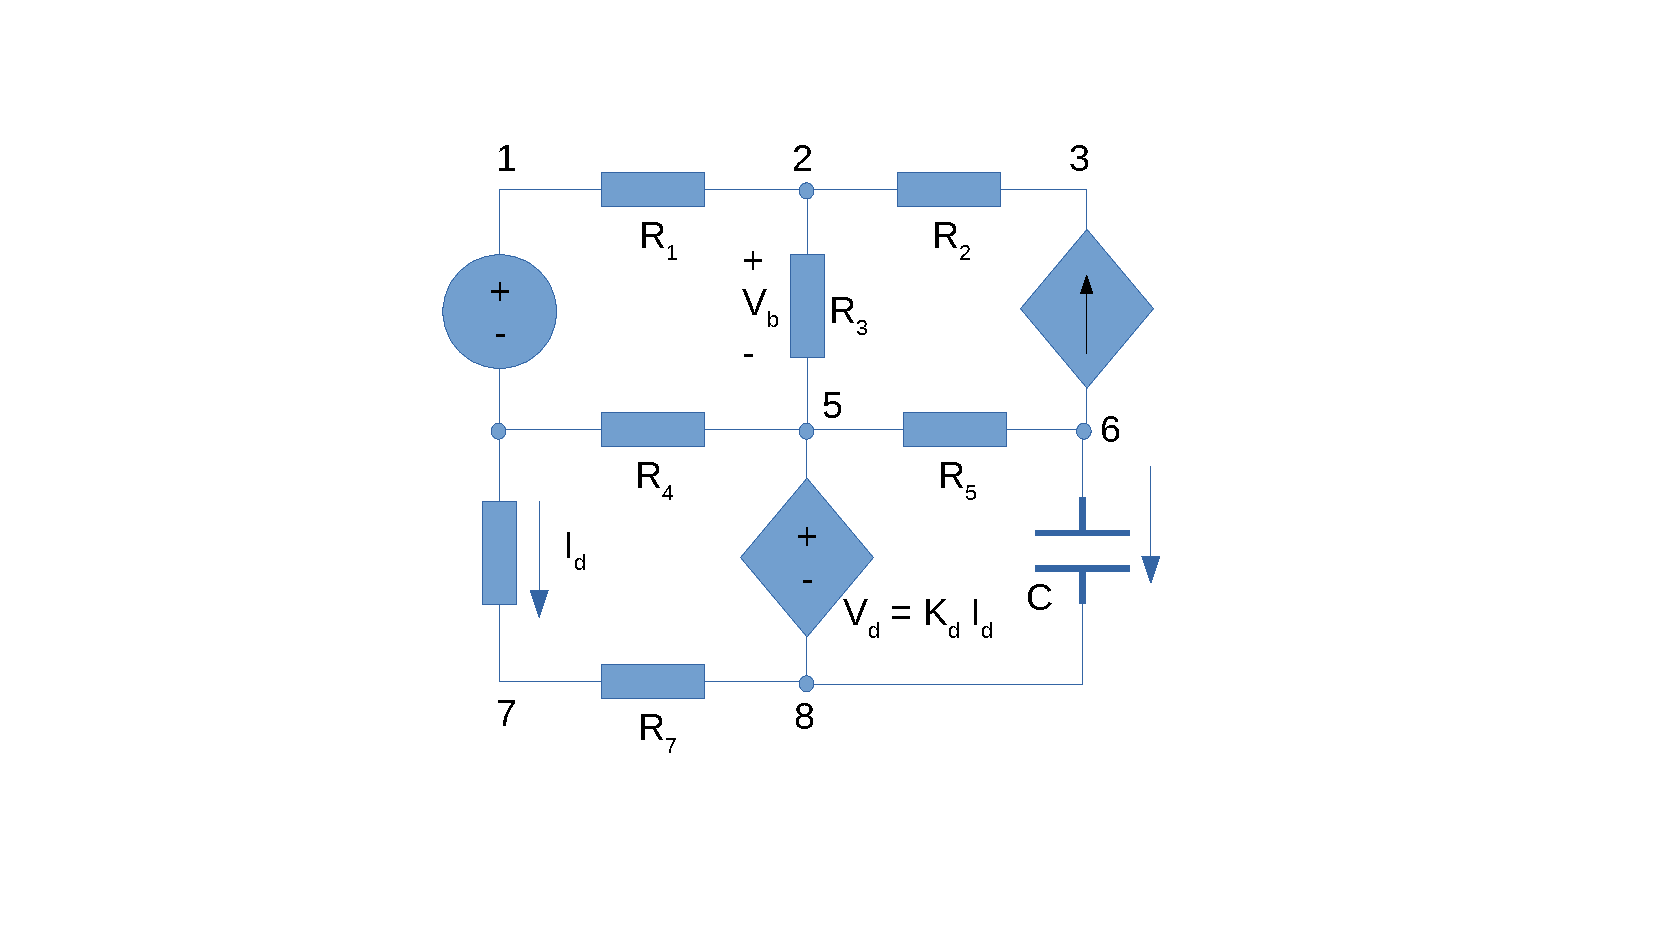
\includegraphics[width=\textwidth]{circuit1.pdf}
\caption{First Circuit}
\label{fig:first}
\end{subfigure}
\begin{subfigure}{0.4\textwidth}
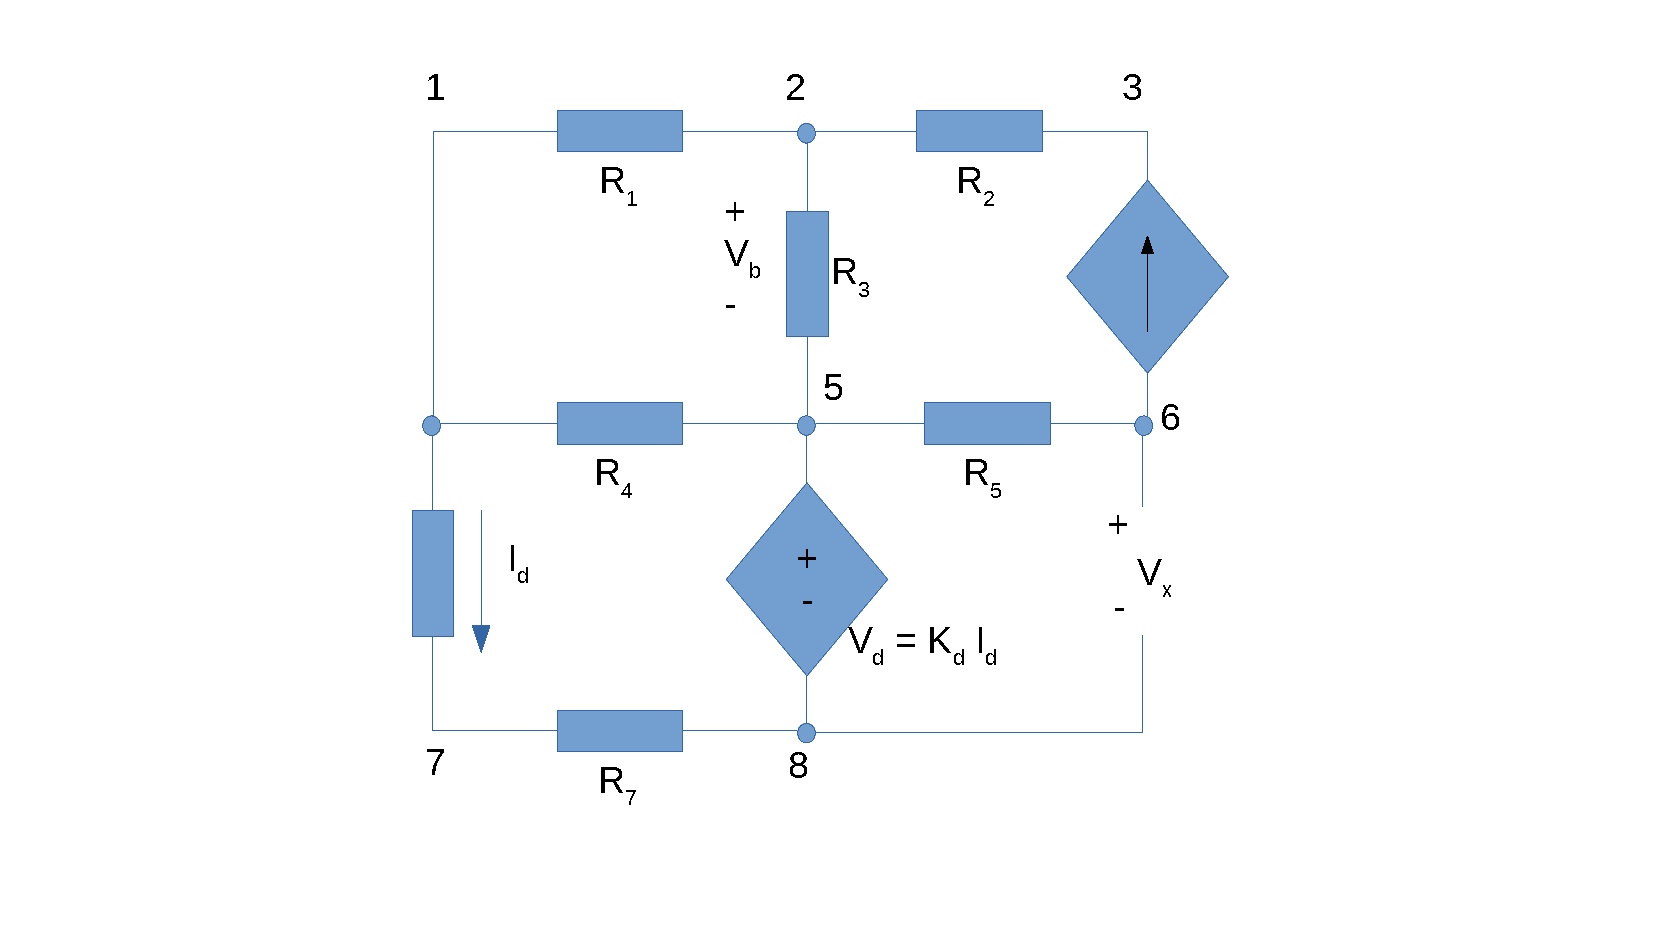
\includegraphics[width=\textwidth]{circuit2.pdf}
\caption{Second Circuit}
\label{fig:second}
\end{subfigure}

\end{figure}


In Section~\ref{sec:analysis}, a theoretical analysis of the circuit is
presented. In Section~\ref{sec:simulation}, the circuit is analysed by
simulation, and the results are compared to the theoretical results obtained in
Section~\ref{sec:analysis}. The conclusions of this study are outlined in
Section~\ref{sec:conclusion}. \\

\pagebreak
